\documentclass[12pt]{article}


\author{Fl\'{a}vio Cruz and Richard Veras}
\title{Assignment 3}

\usepackage{amsmath}
\usepackage{amsfonts}   % if you want the fonts
\usepackage{amssymb}    % if you want extra symbols
\usepackage{savetrees}
\usepackage{algorithmic}
\usepackage{graphicx}
\usepackage{listings}


\begin{document}
\maketitle

\section{Dead Code Elimination}

\begin{itemize}
   \item Direction: Backwards
   \item Meet operator: Intersection.
   \item Lattice elements: Variables defined in the module (true values are faint variables).
   \item Top value: Empty set.
   \item Bottom value: All variables in the module.
   \item Initialization: Using the bottom value (all variables).
   \item Transfer function: $F(x) = X - (ReturnsPrintsControlGlobal \cup Assignments(X))$, where $ReturnsPrintsControlGlobal$ are variables used in control structures, function calls, returns and global variables and $Assignments(X)$ are variables that are used at the right side of assignments of non-faint variables.
\end{itemize}

\subsection{Implementation}

The implementation is very straightforward and follows what was described previously.
We use the \texttt{Variables} class to name all our variables and to generate the universal set (it is also helpful for debugging purposes). For the transfer function, we go over each instruction in a block and apply the required action for each instruction.
For example, for a \texttt{load} instruction, we check if the left hand side is not faint, and, if that's the case, we turn the variable in the right hand side into a non-faint variable. When branches or function calls appear we simply make all the variables involved as non-faint, because something important may be done inside that function and we don't want to delete function calls at all. The exception is when we find a read only function, in that case, we use the same strategy as for simple operations (like +).

An important implementation detail is how we handle arrays. Problems arise when something is stored into the array and the array itself may be used elsewhere (for example, for branches). When some element of the array is changed, a \texttt{store} instruction is used but the value is not propagated, which turns such instruction values as faint and thus can destroy the correctness of the program. In the transfer function, we run a backwards pass over the list of instructions and store to \texttt{arrays} the values of the arrays that are considered non-faint. Then, we turn non-faint \texttt{getelementptr} instructions and corresponding
stores for such arrays into non-faint and finally, we run a final backwards pass to force all the intermediate instructions and values to be marked as non-faint.

Once all the faint variables have been located, we do traverse all the instructions and add those that are deemed for deletion into a queue. Finally, we just go over the queue and delete all the instructions.

\subsection{Experimental Results}

For all the programs below, we used an unoptimized version and an optimized version using our pass. We executed the programs 3 times and then we used the average execution time. Times are in milliseconds.

We used three different programs:

\begin{itemize}
   \item faint.c: the original with some alterations (more loops).
   \item multiple.c: same as faint.c, but uses many array instructions.
   \item float.c: same as faint.c, but uses floating point operations.
\end{itemize}

\begin{center}
    \begin{tabular}{ | l | l | l | l |}
    \hline
    Program & DCE & Unoptimized & Speedup over unoptimized \\ \hline
    faint.c & 300 & 415 & 1.38 \\ \hline
    multiple.c & 534 & 579 & 1.08 \\ \hline
    float.c & 588 & 906 & 1.54 \\ \hline
    \hline
    \end{tabular}
\end{center}

\section{Loop Invariant Code Motion}
Our implementation of Loop Invariant Code motion, builds upon the iterative
framework that we started in the last assignment and extends upon it by
allowing domains other than instructions and variables, namely basic
blocks. In order to fully implement this optimization we had construct several
other analysis phases which included: reaching definitions, dominator graphs,
depth first search on the dominator graph, a loop invariant detection phase as
well as a phase to apply the actual transformation.

As far as experimental results go, this pass is able to effectively find
opportunities for LICM and apply the proper transformation.

\section{Register Allocation}

\subsection{Coloring with 4 registers}

\begin{figure}[!htbp]
    \centering
    \caption{Determining live ranges and merged live ranges.}
    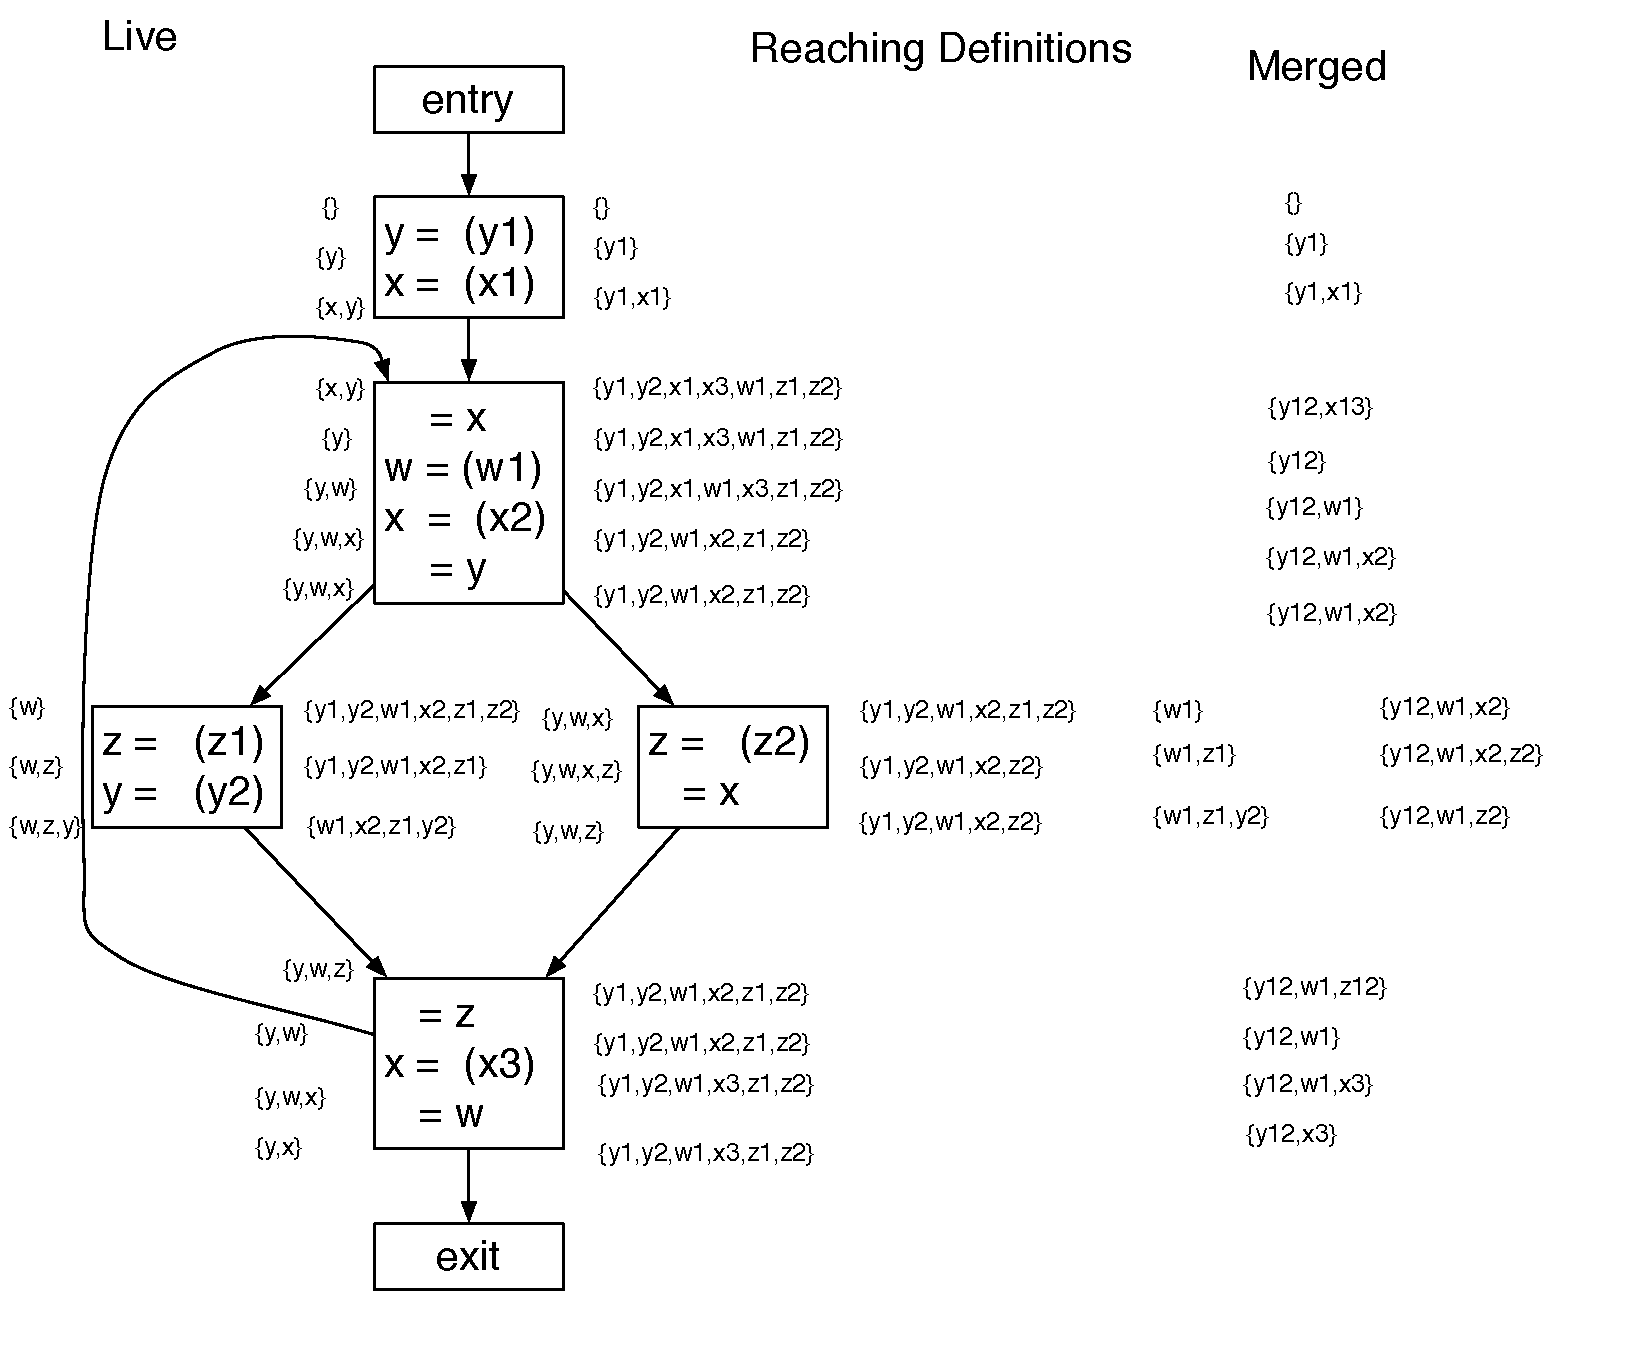
\includegraphics[scale=0.50]{register_allocation1.pdf}
    \label{fig:regalloc1}
\end{figure}

\clearpage

\begin{figure}[!htbp]
    \centering
    \caption{Building the interference graph.}
    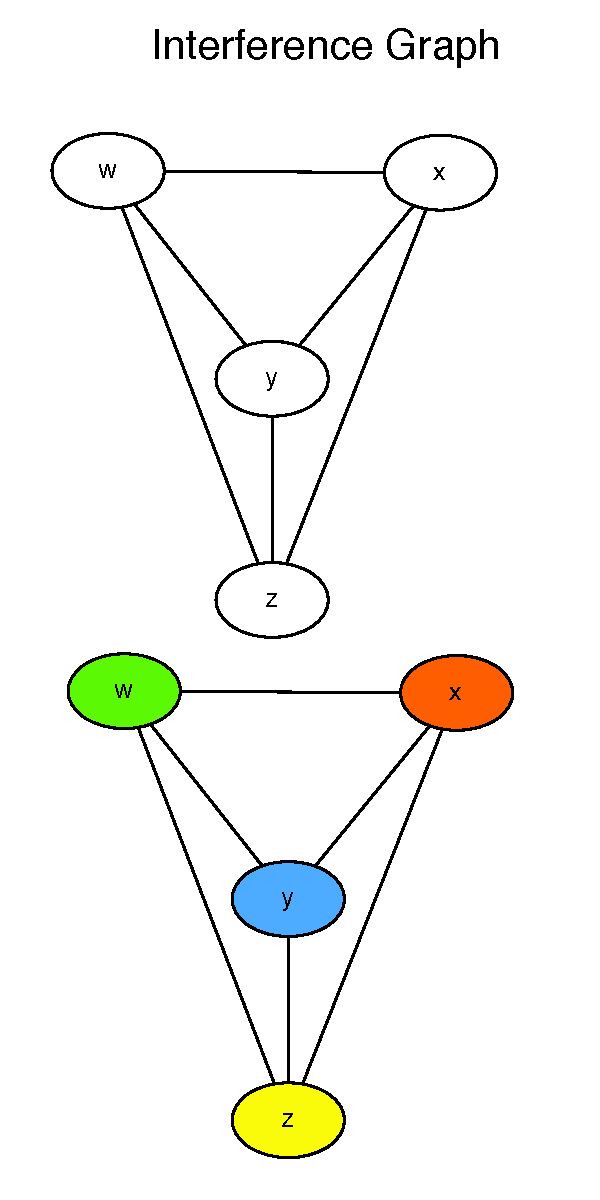
\includegraphics[scale=0.60]{register_allocation2.pdf}
    \label{fig:regalloc2}
\end{figure}

\clearpage

\begin{figure}[!htbp]
    \centering
    \caption{Rewriting the code.}
    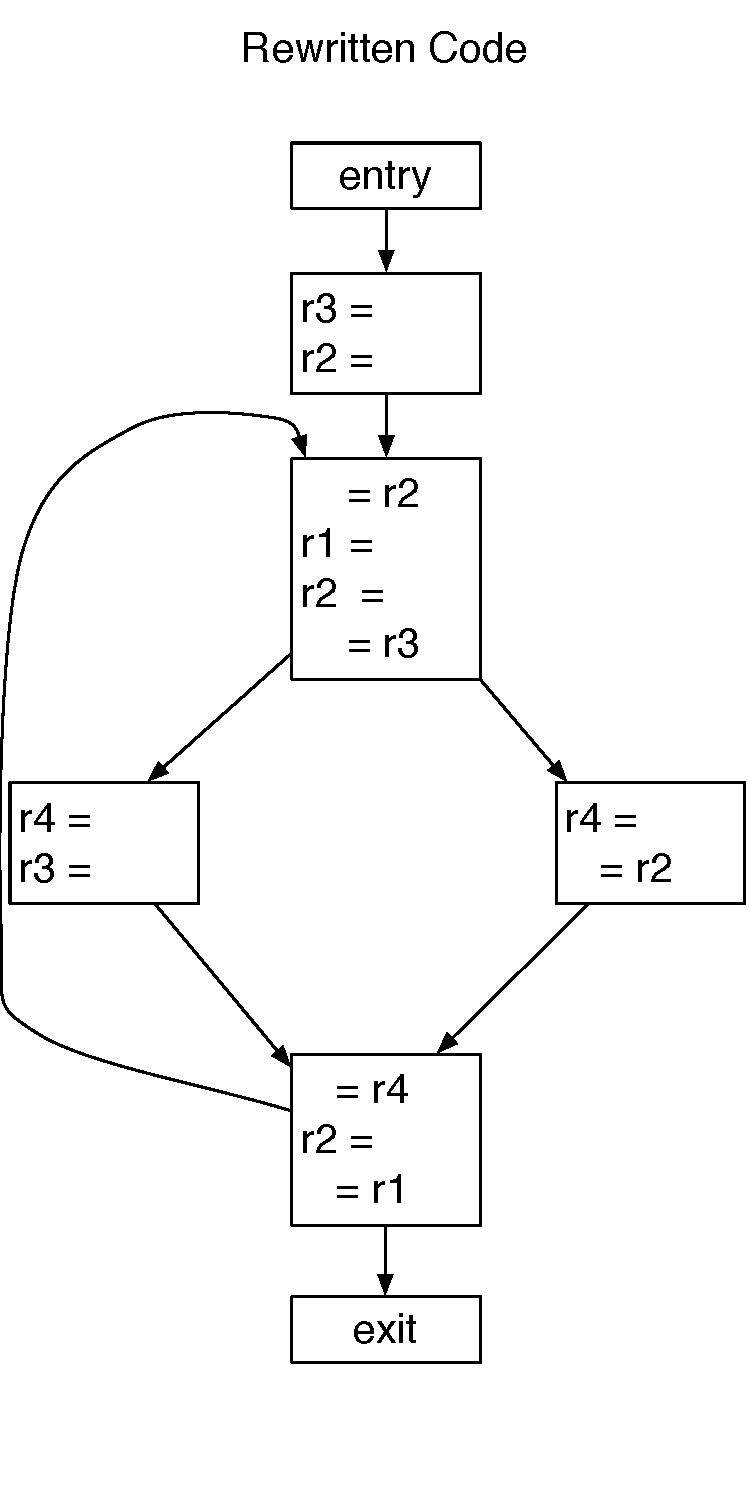
\includegraphics[scale=0.50]{register_allocation3.pdf}
    \label{fig:regalloc3}
\end{figure}

\subsection{Coloring with 3 registers}

No, it's not possible to color the graph using only 3 colors! We have to spill some register to memory.
We can use different approaches to split one register to memory. We will use a simple heuristic (from class),
where we compute the cost of spilling each variable, namely:

$\mathtt{cost} = [(\# \mathtt{defs} + \mathtt{uses}) * 10^{\mathtt{loop-nest-depth}}]/\mathtt{degree}$

We know that $\mathtt{loop-nest-depth} = 1$ for all variables.

\begin{center}
    \begin{tabular}{ | l | l | l | l | l | l |}
    \hline
    Variable & Uses & Defs & Degree & Cost \\ \hline
    w & 1 & 1 & 3 & 6.6 \\ \hline
    x & 2 & 3 & 3 & 16.6 \\ \hline
    y & 1 & 2 & 3 & 10.0 \\ \hline
    z & 1 & 2 & 3 & 10.0 \\ \hline
    \hline
    \end{tabular}
\end{center}

The variable with the least cost is $w$, therefore we will spill $w$ to memory.

\section{Scheduling}
\subsection{Scheduling}
{\tiny
\begin{tabular}{ |r |c c c c|c c c c|c c c c|c c c c|c c c c|c c c c|c c c c|c
    c c c|}
  \hline
  & 0 & & & &4& & & &8& & & &12& & & &16& & & &20& & & &24& & & &28& & & \\
  \hline
  1 &F&D&E&M&M&W& & & & & & & & & & & & & & & & & & & & & & & & & & \\
  2 &F&D&-&E&M&M&W& & & & & & & & & & & & & & & & & & & & & & & & & \\
  3 & &F&D&-&-&-&-&E&E&E&E&E&M&W& & & & & & & & & & & & & & & & & & \\
  4 & &F&D&-&-&-&-&E&M&-&-&-&-&W& & & & & & & & & & & & & & & & & & \\
  \hline
  5 & & &F&D&E&M&M&-&-&-&-&-&-&-&W& & & & & & & & & & & & & & & & & \\
  6 & & &F&D&E&-&M&M&-&-&-&-&-&-&W& & & & & & & & & & & & & & & & & \\
  7 & & & &F&D&-&-&-&-&-&-&-&-&-&-&E&M&W& & & & & & & & & & & & & & \\
  8 & & & &F&D&-&-&-&-&-&-&-&-&-&-&E&M&W& & & & & & & & & & & & & & \\
  \hline
  9  & & & & &F&D&E&M&-&-&-&-&-&-&-&-&-&-&W& & & & & & & & & & & & & \\
  10 & & & & &F&D&-&-&-&-&-&-&-&-&-&E&E&E&M&W& & & & & & & & & & & & \\
  11 & & & & & &F&D&-&-&-&-&-&-&-&-&-&-&-&E&M&W& & & & & & & & & & & \\
  12 & & & & & &F&D&-&-&-&-&-&-&-&-&-&-&-&-&E&M&W& & & & & & & & & & \\
  \hline
  13 & & & & & & &F&D&-&-&-&-&-&-&E&M&-&-&-&-&-&-&-&-&W& & & & & & & \\
  14 & & & & & & &F&D&-&-&-&-&-&-&-&-&-&-&-&-&-&-&E&M&W& & & & & & & \\
  15 & & & & & & & &F&D&-&-&-&-&-&-&-&-&-&E&M&-&-&-&-&-&W& & & & & & \\
  \hline

\end{tabular}

}


\section{Code}

\subsection{Framework}

\begin{itemize}
   \item IterativeFramework.cpp

   {\tiny \lstinputlisting{../DCE/IterativeFramework.cpp}}
   
   \item IterativeFramework.hpp
   
   {\tiny \lstinputlisting{../DCE/IterativeFramework.hpp}}
   
   \item Variables.hpp
   
   {\tiny \lstinputlisting{../DCE/Variables.hpp}}
   
   \item Variables.cpp
   
   {\tiny \lstinputlisting{../DCE/Variables.cpp}}

   \item BlockVariables.hpp

   {\tiny \lstinputlisting{../LICM/BlockVariables.hpp}}

   \item BlockVariables.cpp

   {\tiny \lstinputlisting{../LICM/BlockVariables.cpp}}

   
\end{itemize}

\subsection{DCE}

{\tiny \lstinputlisting{../DCE/DCE.cpp}}

\subsection{DCE Test Cases}

\begin{itemize}
   \item sqrt.c
   
   {\tiny \lstinputlisting{../DCE/sqrt.c}}
   
   \item cast.c
   
   {\tiny \lstinputlisting{../DCE/cast.c}}
   
   \item faint.c
   
   {\tiny \lstinputlisting{../DCE/faint.c}}
   
   \item for-fi.c
   
   {\tiny \lstinputlisting{../DCE/for-fi.c}}
   
   \item if.c
   
   {\tiny \lstinputlisting{../DCE/if.c}}
   
   \item simple.c
   
   {\tiny \lstinputlisting{../DCE/simple.c}}
   
   \item unreachable.c
   
   {\tiny \lstinputlisting{../DCE/unreachable.c}}
   
   \item coiso.c
   
   {\tiny \lstinputlisting{../DCE/coiso.c}}
   
   \item float.c
   
   {\tiny \lstinputlisting{../DCE/float.c}}
   
   \item global.c
   
   {\tiny \lstinputlisting{../DCE/global.c}}
   
   \item multiple.c
   
   {\tiny \lstinputlisting{../DCE/multiple.c}}
   
   \item switch.c
   
   {\tiny \lstinputlisting{../DCE/switch.c}}
   
   \item vector.c
   
   {\tiny \lstinputlisting{../DCE/vector.c}}
\end{itemize}



\subsection{Framework}

\begin{itemize}
   \item IterativeFramework.cpp

   {\tiny \lstinputlisting{../LICM/IterativeFramework.cpp}}

   \item IterativeFramework.hpp

   {\tiny \lstinputlisting{../LICM/IterativeFramework.hpp}}

   \item Variables.hpp

   {\tiny \lstinputlisting{../LICM/Variables.hpp}}

   \item Variables.cpp

   {\tiny \lstinputlisting{../LICM/Variables.cpp}}

   \item BlockVariables.hpp

   {\tiny \lstinputlisting{../LICM/BlockVariables.hpp}}

   \item BlockVariables.cpp

   {\tiny \lstinputlisting{../LICM/BlockVariables.cpp}}

\end{itemize}

\subsection{LICM}

{\tiny \lstinputlisting{../LICM/LICM.cpp}}

\subsection{LICM Test Cases}

\begin{itemize}
   \item loop.c

   {\tiny \lstinputlisting{../LICM/loop.c}}

   \item other.c

   {\tiny \lstinputlisting{../LICM/other.c}}
\end{itemize}

\end{document}
